Para poder dar una correcta definición de qué es una burbuja económica, se han de tener claros dos conceptos fundamentales en economía: el valor y la sobrevaloración de los precios de un bien o servicio. 
\section{El valor y la sobrevaloración} 
El valor es un concepto subjetivo de difícil definición, ya que cada individuo tiene diferentes perspectivas según la postura en la que se encuentre. 

En primer lugar, hay que añadir que es una variable que influye a la hora de llevar a cabo transacciones donde también hay involucrados múltiples agentes de toda la cadena productiva y comercial, como son los propietarios, los proveedores, las empresas y los vendedores. 

Se plantea una cuestión, \emph{¿Cuál es el significado de valor en el contexto de los negocios?} Según la Real Academia de la Lengua Española define valor como \emph{el grado de utilidad o aptitud de las cosas, para satisfacer las necesidades o  proporcionar bienestar o deleite}. Por otro lado, el conocido autor en materia económica Michael Porter (1.980), define el valor como \emph{una cadena vertical que abarca desde los proveedores de recursos hasta los compradores finales teniendo en cuenta a las empresas y sus servicios. El valor se crea a lo largo de esta cadena sufriendo variaciones debidas a los diferentes agentes. Estos agentes son los proveedores, las empresas y los compradores}	\footnote{Fuente: Porter (1.996)} . Esta cadena se puede observar en la Figura \ref{fig:Cadena de agentes}.

\begin{figure}[!h]
	\caption{Cadena de agentes}
	\centering 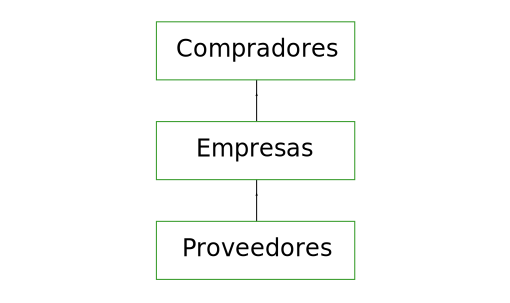
\includegraphics[width=150mm]{capitulos/graficos/cadenaAgentes} 
	\label{fig:Cadena de agentes} 
	
		\footnotesize
		Fuente: Brandenburguer, \& Harbone, (1.996)


\end{figure}

El valor añadido viene definido por el autor Brandenburguer (1.996) como, \emph{el valor creado a lo largo del proceso. Desde los proveedores hasta los compradores, teniendo en cuenta la cantidad y el precio que estos están dispuestos a adquirir o a pagar respectivamente, no sólo por un producto o servicio que cubra las necesidades, si no por un producto que aporte algún factor añadido} \footnote{Fuente: Brandenburguer, \& Harbone, (1.996)} 

Continuando la teoría de Brandenburguer y Harbone (1.996), en un modelo simplificado, el valor viene definido por la voluntad de pago del comprador y por el coste de oportunidad del vendedor, siguiendo una ecuación: 

\begin{gather*}
    Valor = voluntad - coste
\end{gather*}

Como se mencionó al comienzo del epígrafe, la definición de valor parece abstracta y en algunos contextos lo es. También es complicado realizar un cálculo por lo que se puede plantear otra cuestión, \emph{¿Cómo se determina el valor apropiado para cada agente de la cadena?} Se puede observar de una manera rápida y visual gracias a la Figura \ref{fig:Cadena de valor}.

\begin{figure}[!h] 
\caption{Cadena de valor} 
\centering \includegraphics[width=150mm]{capitulos/graficos/cadenaValor} 
\label{fig:Cadena de valor} 

	\footnotesize
	Fuente: Brandenburguer, \& Harbone, (1.996)

\end{figure}

Por lo tanto, se puede concluir que debido a la existencia de multitud de oferta, la diversidad de compradores tiene varias opciones de compra. De este modo, tiene que existir congruencia entre compradores y vendedores llegando a alcanzar un trato positivo para ambas partes y de este modo alcanzar el equilibrio de mercado.

Una vez queda explicado el valor, frente al precio ordinario de un bien o servicio, se ha de plantear otra cuestión, \emph{¿Cómo se puede saber si un bien se encuentra sobrevalorado por los consumidores?} \emph{El valor} es un concepto abstracto y propio de cada individuo tal y como se ha mencionado. Alcanzar su conocimiento de una forma directa con instrumentos económicos, parece un hecho imposible en la actualidad. Por ello, resulta más sencillo realizar estimaciones con precios reales aplicando dos métodos fundamentales establecidos por los autores Brandenburguer y Harbone (1.996) y que tan sólo se mencionaran debido a su complejidad. Por un lado el método de ratios que compara los precios de un bien o servicio con respecto a otro indicador. El resultado se contrasta con otro valor que el mercado lo encasilla en fase de normalidad. Un ejemplo es el ratio del PER. Y por otro lado, el método de residuos de un modelo \emph{X} que consiste en explicar los precios a través de un modelo econométrico teniendo en cuenta variables clásicas tales como el carácter demográfico, tipos de interés, etc. Éste último es un método más costoso que el anterior.

Una vez explicados estos dos conceptos abstractos, se puede comenzar a dar forma a la definición de burbuja económica. 

\section{¿Qué es una burbuja económica?}

El concepto de burbuja económica no está exento de cierta ambigüedad. Si bien existe un razonable acuerdo en asociarlo con un intenso y prolongado aumento en el precio de un activo, seguido por una abrupta y rápida caída del mismo; no hay consenso acerca de cuáles son las causas que provocan la burbuja ni sobre cuál debe ser su definición única y precisa. En particular, no existen límites preestablecidos para determinar hasta qué punto el precio de un activo debe subir y cómo debe subir para que se considere un caso de burbuja económica. 

A este fenómeno en sus orígenes se le denominaba  \emph{manía}. La palabra manía, tiene en cuenta a los individuos o agentes que se introducen en el mercado en el momento en el que éste se encuentra más exaltado por los inversionistas. En ese momento, la venta parcial o total de los activos tiene el fin de comprar más activos para lucrarse en un futuro, es decir, lo que hoy llamaríamos un \emph{proceso especulativo}. La manía concluye cuando algunos individuos o agentes venden los activos al percatarse de que los precios no podrán mantener esa trayectoria ascendente. La caída de precios se produce por el descenso de demanda.

La primera de ellas surgió en Holanda en 1.637 en el mercado del tulipán. Algunos de los tulipanes, como se verá a lo largo del capítulo dos, alcanzaron precios desorbitados. El concepto de esta manía, refleja el hecho de que los individuos adquirían tulipanes a un precio muy alto con la expectativa de venderlos a un precio aún más alto a otro individuo o agente que tuviese una mayor expectativa sobre la evolución futura de los precios. La palabra manía tiene en cuenta también el hecho de que la venta parcial o total de estos tulipanes tiene como fin la compra de más tulipanes para poder cobrar beneficios adicionales, es decir, para llevar a cabo un proceso especulativo. Esta manía finalizó cuando algunos individuos vendieron sus tulipanes ya que creyeron que los precios no podrían mantenerse tan elevados. 

Como se va a poder comprobar a lo largo del presente capítulo, una burbuja económica puede aparecer prácticamente en cualquier lugar del mundo. Por ejemplo han surgido en países como Argentina, Australia, China, Estados Unidos, España, Holanda, Irlanda, Japón, Rumanía, Zimbabwe, etc. También se puede destacar la variedad de materias primas, bienes o servicios que han sido víctima de este fenómeno como por ejemplo los tulipanes, las acciones, el uranio, el rodio, el trigo, los inmuebles, etc. 

Los efectos y resultados a posteriori de la burbuja económica, también pueden variar dependiendo de diferentes factores. Sin embargo, existe una clara evidencia empírica de que las burbujas económicas generan una redistribución de la riqueza entre los diversos agentes de la economía. Es evidente que puede dañar la economía, pero también puede generar una fuerte desviación temporal en cuanto a la tendencia del precio se refiere, o por el contrario incluso en algunos casos podría beneficiar a la economía, como se comprobará a lo largo del presente capítulo, aunque este último aspecto causa controversia en sí mismo. Se pueden demostrar estos hechos beneficiosos con los ejemplos de expansión y proliferación de Internet durante la burbuja punto com, o el Crack de 1.929 en Estados Unidos entre otros, desarrollados a continuación. Estos efectos serán expuestos más adelante.

Retomando la intención de dar una definición apropiada al término burbuja económica no se puede pasar por alto la analogía presentada por uno de los autores principales en la materia, Van Horne (1.985). Este autor presenta un paralelismo entre una burbuja y un globo. De este modo se puede comprender de una forma visual cómo se desarrollan las burbujas. Defiende que una burbuja económica es como un globo que se infla progresivamente y puede realizarlo de dos formas diferentes. El primer caso, es introducir el aire gradualmente impidiendo que éste se desprenda precipitadamente. Y la segunda opción, es que el aire se introduzca rápidamente y haya más probabilidades de que se produzca un pinchazo en el globo, lo que provocaría la explosión de éste y por lo tanto, retomando la burbuja económica, que los precios aumenten repentinamente hasta llegar a un punto en que éstos han de descender. Esto puede suceder de una forma repentina o paulatinamente. Obviamente las consecuencias son muy diferentes según se desarrolle cada caso
.

Llegados a este punto del capítulo, se puede afirmar que la definición teórica que más se asemeja al término de burbuja económica es la de DeMarzo (2.007): \emph{Se define una situación de burbuja en el momento en el que existe un precio de mercado de un activo que es superior a su valor fundamental, siendo el valor fundamental el valor presente de los pagos futuros}. 

\section{Breve cronología de las burbujas económicas más importantes a lo largo de la historia} 
A continuación se van a narrar brevemente algunas de las burbujas económicas históricas más relevantes.
\subsection{La tulipomanía} 
Esta burbuja histórica clásica, desarrollada en profundidad en el capítulo dos, tiene como pieza principal los tulipanes. Esta planta fue importada a Holanda a finales del siglo XVI y no tardó en convertirse rápidamente en un bien caro pero accesible antes de la manía. La locura se desató en el momento en el que algunos tulipanes comenzaron a adquirir diferentes colores en una misma flor y se comenzaron a \emph{sobrevalorar} estos bulbos extremadamente raros \footnote{Se dará explicación detallada acerca de estos tipos de tulipanes en el capítulo dos.} y bellos.

En un principio eran sólo comerciantes los que especularon con el precio futuro de los tulipanes, comprando así, grandes cantidades de éstos mismos con antelación para la temporada siguiente. Pero a medida que los precios aumentaron, gran parte de la población quería ser partícipe introduciéndose en el mercado y empezando a especular con tulipanes. 

\begin{figure}[!h] 
\caption{Nivel de precios de la Tulipomanía} 
\centering 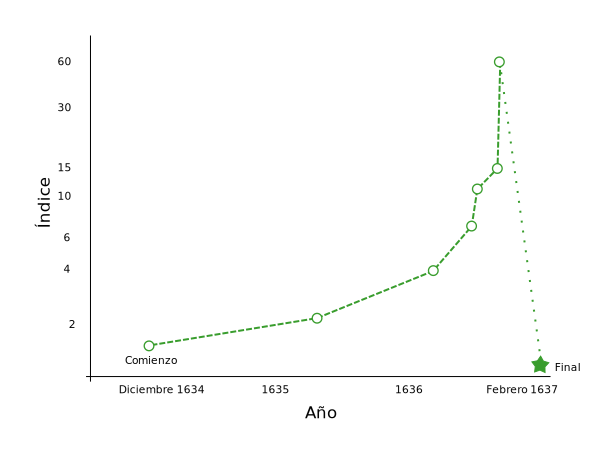
\includegraphics[width=150mm]{capitulos/graficos/TulipBubble} 
\label{fig:Nivel de precios de la Tulipomanía} 

	\footnotesize
	Fuente: Eliot Wave International (1.999)

\end{figure}

Como se puede apreciar en la Figura \ref{fig:Nivel de precios de la Tulipomanía}, el punto álgido de la burbuja tuvo lugar a principios de 1.637, cuando tan solo un bulbo de tulipán \emph{raro}, se vendía por una cantidad equivalente al precio del castillo de un noble. La manía, sumergida en un continuo circuito de retroalimentación negativa, provocó que la deflación del bulbo creciese a un ritmo cada vez más rápido. En escasos días, el pánico reinaba en Holanda y los precios se desvanecieron. Este episodio fue seguido por una severa disminución de la actividad económica de la que se necesitaron muchos años para conseguir la completa recuperación.

\subsection{La Compañía del Mississippi} 

La burbuja de la Compañía del Mississipi será analizada en profundidad en el capítulo tres. 

Se trata de una burbuja económica que se dio en Francia a principios del siglo XVIII y que se desarrolló en paralelo con la burbuja de la Compañía de los Mares del sur en Gran Bretaña. El cerebro que se escondía tras la burbuja del Mississippi era John Law, un financiero escocés que ascendió a los escalones superiores de la hacienda pública francesa a través de su amistad con el Archiduque de Felipe II de Orléans.

Law se convirtió en el primer asesor financiero del gobierno francés y utilizó a este para poder instaurar un banco con la autoridad suficiente como para emitir \emph{dinero papel}; y en segundo lugar, otorgando un monopolio en el mercado a La Compañía del Mississippi. De este modo, a principios de 1.719, esta Compañía absorbió gran cantidad de compañías mercantiles importantes renombrándose \emph{La Compañía de las Indias}. En julio de ese mismo año, la Compañía adoptó el derecho de cobrar todos los impuestos indirectos franceses y en octubre de 1.719 se hizo cargo de la recaudación de impuestos directos.

\begin{figure}[!h] 
\caption{Precio de las acciones de la Compañía del Mississippi 1.719 - 1.720} 
\centering \includegraphics[width=150mm]{capitulos/graficos/preciosAccionesIndias} 
\label{fig:PrecioAccionesCompaniaMississippi} 

	\footnotesize
	Fuente: Thornton, H (2.010)

\end{figure}

Como se puede comprobar en la Figura \ref{fig:PrecioAccionesCompaniaMississippi} , la explosiva demanda de acciones de la Compañía de las Indias, provocó que la cantidad total de dinero papel que el banco expedía, aumentase en un 186 por ciento en un año. Pero en enero de 1.720, las acciones de la Compañía comenzaron a caer en picado ya que algunos inversores decidieron retomar el antiguo sistema de monedas de oro y plata. Las acciones de la Compañía, se devaluaron y el dinero papel lo hizo en mayor medida alcanzando el 50 por ciento en mayo de 1.720 y creando pánico entre los inversores. Estos inversores se arruinaron y a finales de 1.720, John Law fue visto como un estafador y escapó de Francia. El colapso del banco nacional y la Compañía de las Indias coincidió con el estallido de la burbuja de los Mares del Sur de Gran Bretaña.

\subsection{La Compañía de los Mares del Sur}  

El estudio en profundidad de esta burbuja económica se desarrollará en el capítulo cuatro.

En el año 1.711, en la ciudad de Londres, se fundó la Compañía de los Mares del Sur, la cual ayudó a restaurar la fe en la solvencia del gobierno mediante la compra de diez millones de libras en bonos del gobierno. La Compañía, recibió el monopolio del comercio inglés de los Mares del Sur. Había un gran entusiasmo acerca de los beneficios que se podían alcanzar desarrollando un comercio con América, ya que la Compañía siempre se las arregló para tener una buena propaganda positiva y sus perspectivas de comercio mejoraron cuando Gran Bretaña puso fin a la guerra con España y México. La compañía tenía el favor distintivo del gobierno y tanto los inversionistas como el pueblo creían que existían riquezas potenciales que se llevarían a cabo con en el nuevo comercio de oro, plata, algodón y lana en América. En 1.720, se propusieron aumentar la reputación de la Compañía ofreciéndose a financiar la totalidad de la deuda nacional, que ascendía a 31 millones de libras. Este hecho inició la especulación sobre el precio de las acciones. 

Como se puede observar en la Figura \ref{fig:PrecioAccionesMaresSur}, el 7 de abril tras ser publicado un proyecto de ley en el Parlamento, el precio de las acciones aumentaron rápidamente de 130 a 300 libras. Con el tiempo, el precio de las acciones aumentó hasta alcanzar las 1.000 libras. Llegado a ese punto, el precio de las acciones no tenía concordancia con la situación real de la empresa y los directores, y demás individuos influyentes, decidieron vender sus participaciones durante el verano.

\begin{figure}[!h] 
\caption{Precio de las acciones de la Compañía de los Mares del Sur 1.717 - 1.722} 
\centering 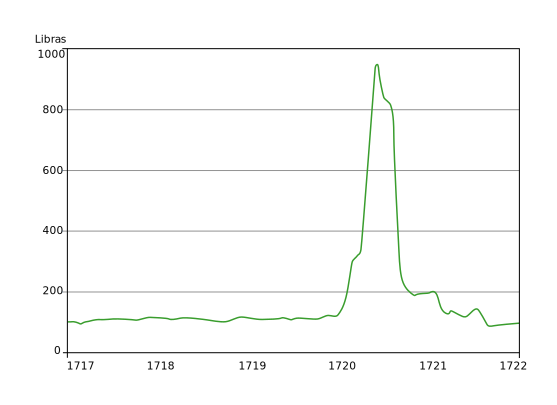
\includegraphics[width=150mm]{capitulos/graficos/SouthSeaStockPrice} 
\label{fig:PrecioAccionesMaresSur} 

	\footnotesize
	Fuente: L. Neal (1.990)

\end{figure}

La noticia llegó a oídos de la multitud y el pánico se instaló en el pueblo, provocando que el precio se derrumbase. Entre los grandes perjudicados de la burbuja de los Mares del Sur se encuentra Isaac Newton, quien exclamó: \emph{Puedo calcular los movimientos de los cuerpos celestes, pero no la locura de la gente}. 

Se trata de una historia muy similar a la de la Compañía de los Mares del Sur, que ocurrió en el mismo período de tiempo en Francia. Durante este período de tiempo hubo casos masivos similares de empresas que comenzaban a prometer grandes recompensas y en algunas ocasiones se trataba de fraudes donde los propietarios se quedaban con el dinero de las inversiones.


\subsection{La manía del ferrocarril}  

Al mismo tiempo que se gestaba la Revolución Industrial en Gran Bretaña, surgió la necesidad de crear un gran sistema de transporte tanto para la industria como para la población. Así, el ferrocarril parecía una necesidad imperiosa. En un principio, cientos de empresas ofrecieron presupuestos al Parlamento para que éste los aprobase, un total de 272 fueron aptos. Finalmente, se tuvieron en cuenta todos los proyectos de todas las empresas ferroviarias y se creó una propuesta global de construcción de 15.300 kilómetros de vía. Por otro lado, en el país, las familias con poder adquisitivo medio iban en aumento al mismo tiempo que una gran parte de la población sabía leer y escribir. Este sector de la población, también poseía ahorros acumulados y se sentían dispuestos a invertir. Además, el Banco de Inglaterra redujo los tipos de interés y el gobierno promovió en gran medida los proyectos ferroviarios.

Seis mil individuos se convirtieron en inversores del ferrocarril haciéndose con un gran número de acciones pagando un depósito. La Manía del ferrocarril fue víctima de una verdadera campaña publicitaria por parte del gobierno y de algunas empresas poco solventes. En el año 1.845, la inviabilidad de muchos proyectos se hizo evidente. El Banco de Inglaterra, no tardó en elevar los tipos de interés a finales de ese año y muchas empresas se quedaron sin fondos. Las perspectivas de rentabilidad de las inversiones desaparecieron.

\begin{figure}[!h] 
\caption{La Railmania} 
\centering 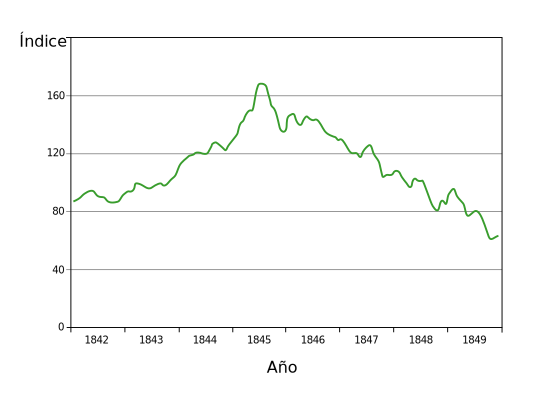
\includegraphics[width=150mm]{capitulos/graficos/LaRailmania} 
\label{fig:La Railmania} 

	\footnotesize
	Fuente: Global Financial Data, Inc

\end{figure}

A principios de 1.850 sobrevivieron las principales compañías ferroviarias. Sin embargo, en este caso no hubo un efecto tan relevante en la población tras el estallido de la burbuja como algunos autores señalan. Entre ellos, Wolmar, (2.007). El sistema ferroviario británico se expandió enormemente durante el período de euforia inversionista debido al frenesí especulativo que atrajo importantes cantidades de capital privado que eran necesarios para la construcción del ferrocarril, además de que los bancos estaban dispuestos a prestar.

Un total de 10.000 kilómetros se construyeron como resultado de proyectos autorizados entre 1.844 y 1.846. Es interesante compararlo con la red ferroviaria moderna del Reino Unido, que abarca un total de 34.000 kilómetros. Este hecho da una idea de la importante construcción realizada en un corto período de tiempo.

\subsection{El Crack del 29}  

En cuanto a los mercados modernos, se tiene que mencionar el gran mercado alcista de los Estados Unidos que se derrumbó en 1.929. Está considerada como una de las mayores burbujas bursátiles de todos los tiempos.

La explicación más aceptada de lo ocurrido en el mercado de valores de Estados Unidos es la dada por Galbraith (1.954), en la que señala que la burbuja se fue gestando durante el rápido crecimiento y expansión del crédito en forma de préstamos que los inversores no pagaban. Sin embargo, hay otros estudios que afirman el hecho de la inexistencia de burbuja económica durante este período, ratificando que los precios de las acciones reflejan los valores fundamentales de acuerdo con los estudios econométricos, en este caso, el autor relevante que defiende esta postura es Hamilton (1.986). Una versión revisada y completa de este estudio apunta a una combinación de factores generadores de la burbuja económica que no eran tan sólo los mencionados por Galbraith. Estos factores no pueden ser detectados con los datos econométricos ya que el periodo de tiempo transcurrido fue muy corto según establece White (1.990).

A partir de 1.928, la especulación en el mercado de valores se convirtió en un pasatiempo nacional. De 1.922 a 1.929, el PIB creció a una tasa anual del 4,7 por ciento y el desempleo descendió un 3,7 por ciento. Grandes condiciones económicas se estaban propiciando. Por ejemplo la aparición de las grandes empresas comerciales e industriales, las economías a escala y la gestión moderna. Las empresas emitían acciones para financiar nuevas naves y equipos. Los bancos comerciales comenzaron a dedicarse a la banca de inversión creando filiales. El número de afiliados creció de 10 a 114 entre 1.922 y 1.931, según indica Peach (1.941) en su estudio. Gran parte de los nuevos inversores que participaron en el mercado de valores, carecían de experiencia, facilitando así la creación de la burbuja. Entre el 3 de marzo de 1.928 y el 3 de septiembre de 1.929 la participación en los principales valores que cotizaban en Wall Street aumentó del 87 por ciento hasta 434,5 por ciento como según afirma Malkiel (1.973).

\begin{figure}[!h] 
\caption{El crack de 1.929} 
\centering 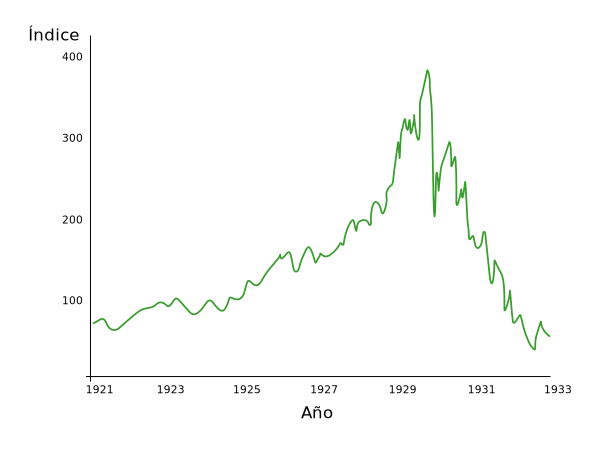
\includegraphics[width=150mm]{capitulos/graficos/1929Bubble} 
\label{fig:El crack de 1.929} 

	\footnotesize
	Fuente: Elaboración propia a partir de los datos recuperados en Dow Jones Industrials (2.012)

\end{figure}

En el mes de septiembre del año 1.929, y tal como se puede apreciar en la Figura\ref{fig:El crack de 1.929}, hubo más días malos que buenos. Aun así, los banqueros y los funcionarios del gobierno aseguraron al país que no había motivo de preocupación. El 21 de octubre de 1.929, todo estaba preparado para el colapso del mercado. Las caídas de las cotizaciones bursátiles llevaron a exigir más garantías a los clientes que habían comprado acciones con dinero prestado. Estos clientes se vieron obligados a vender sus pertenencias para hacer frente a la deuda adquirida en el pasado. Esta caída de los precios realizó un ajuste de los márgenes de dinero prestados y una ola vendedora de acciones. 

El 24 de octubre de 1.929, más tarde llamado \emph{Jueves Negro}, muchas de las acciones vieron reducidos sus precios en un 25 por ciento durante dos horas. Al día siguiente, el presidente Herbert Hoover lanzó un mensaje al pueblo en el que decía: \emph{El negocio fundamental del país, se encuentra sobre una base sólida y próspera}.

El martes, 29 de octubre 1.929, se considera como uno de los días más catastróficos de la historia de la Bolsa de Valores de Nueva York. La caída de la bolsa fue seguida por una intensa y devastadora depresión, una de las más importantes en la historia del país. El estallido sucedió en sí, debido a las políticas llevadas a cabo, que como consecuencia, elevaron las tasas de interés para castigar a los especuladores.

En contraposición a la idea de que el Crack del 29 fue una burbuja económica, se encuentra la opinión de Bierman Jr (1.991), quien defiende que las acciones no fueron demasiado caras durante el año 1.929 debido a que parecía que la economía seguía una dinámica próspera.

\subsection{La burbuja económica de Japón}  

Durante la década de los 80, Japón comenzó a crecer económicamente durante un largo periodo de tiempo y mantuvo estable la inflación con la excepción del precio de los activos inmobiliarios, que aumentaron rápidamente.

Del año 1.955 hasta 1.990, el valor de los inmuebles japoneses aumentó más de 75 veces, situando así el valor total de todos los bienes mobiliarios, cerca de los 20 billones de dólares, el equivalente a más del 20 por ciento de la riqueza del mundo, según confirma Malkiel (1.973).

\begin{figure}[!h] 
\caption{Precio de las acciones de la Burbuja Japonesa} 
\centering 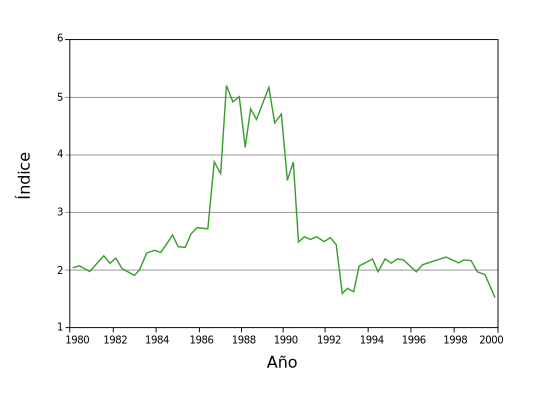
\includegraphics[width=150mm]{capitulos/graficos/JapaneseStockMarketBubble} 
\label{fig:Precio de las acciones de la Burbuja Japonesa} 

	\footnotesize
	Fuente: Estimaciones del banco Morgan Stanley

\end{figure}

Como se puede observar en la Figura \ref{fig:Precio de las acciones de la Burbuja Japonesa}, la burbuja económica se sitúa entre 1.987 y 1.990. Fue entonces cuando los precios de acciones, los precios de los terrenos y los precios de los bienes comenzaron a comportarse de una forma diferente a la habitual. El punto más alto, se alcanzó en diciembre de 1.989, cuando las acciones japonesas tuvieron un valor total de mercado de 4 billones de dólares, casi 1,5 veces el valor de todas las acciones de Estados Unidos y cerca del 45 por ciento del mundo.

Las causas del surgimiento de la burbuja económica pueden ser identificadas como factores interconectados que aumentaron las expectativas optimistas de la economía. Según Shiratsuka, (2.003) el comportamiento agresivo de las instituciones financieras, el progreso de la desregulación financiera, la gestión inadecuada del riesgo por parte de las instituciones financieras, la introducción del Acuerdo de Capital, la flexibilización monetaria prolongada, los impuestos y las regulaciones sesgadas, aceleraron la subida de los precios, provocaron un exceso de confianza y euforia y concentraron sus esfuerzos en convertir a Tokio en un centro financiero internacional. 

Un punto fundamental a tener en cuenta, es que los tipos de interés continuaron siendo bajos a pesar de la expansión económica de la época, lo que contribuye al crédito fácil y barato.

Como en otros casos de burbujas económicas, la disminución de la rentabilidad hizo que los agentes revisasen sus expectativas provocando el desplome del mercado de valores y del mercado inmobiliario. El colapso de esta burbuja en Japón, tuvo profundos efectos en el sistema financiero y en la economía japonesa, por lo que debilitó todo el sistema financiero y fue seguida por una severa recesión que duró hasta el siglo siguiente. 

Hay un cierto paralelismo entre esta burbuja y la de 1.929 en Estados Unidos anteriormente descrita. Principalmente por el extremo colapso que las ciudades vivieron en ambos casos. 

\subsection{La crisis asiática}   

Los países más afectados durante este boom y colapso fueron: Corea del Sur, Filipinas, Indonesia, Malasia y Tailandia.

Entre 1.980 y 1.990, las tasas de interés en las economías desarrolladas, fueron relativamente bajas en comparación con las tasas de interés de las economías en desarrollo de Asia. Este hecho generó un gran flujo de dinero que dio un impulso a las economías regionales de Asia. Los llamados \emph{dragones asiáticos}, lograron tasas de crecimiento del PIB que abarcaban del 12 por ciento al 8 por ciento. Sin embargo, según Krugman (1.994), este crecimiento estaba basado casi puramente en un elevado déficit en sus cuentas corrientes, lo que se tradujo en un endeudamiento externo y a un apalancamiento de la economía debido al riesgo del cambio de divisas. 

Entre 1.995 y 1.996 las exportaciones asiáticas aumentaban a tasas muy elevadas, un 20 por ciento. Se ha de tener en cuenta, que las exportaciones son una variable muy importante en la economía asiática ya que suponen un porcentaje muy alto del PIB nacional. Por ejemplo, en Corea del Sur y Tailandia, el porcentaje asciende al 40 por ciento. En 1.997, las exportaciones comenzaron a descender debido a la revaluación de las diferentes monedas asiáticas, lo que hacía que aumentase la presión entre las monedas, perjudicando así a la asiática y provocando una pérdida de competitividad con el resto de países. Al mismo tiempo, los Estados Unidos se recuperaban de una recesión y comenzaron a subir los tipos de interés. Esto, provocó que las inversiones del país fuesen más atractivas y además se producía una apreciación del dólar. Infinidad de capitales comenzaron a salir y la especulación se volvió pesimista sobre las monedas asiáticas. Todo el proceso de colapso se describe con tan sólo una palabra: \emph{pánico}. 
Se puede comprobar este crecimiento en la Figura \ref{fig:AsianCrisis}.

\begin{figure}[!h] 
\caption{Flujo de capital de los países asiáticos emergentes 1991 - 2010 (Porcentaje según el PIB)} 
\centering 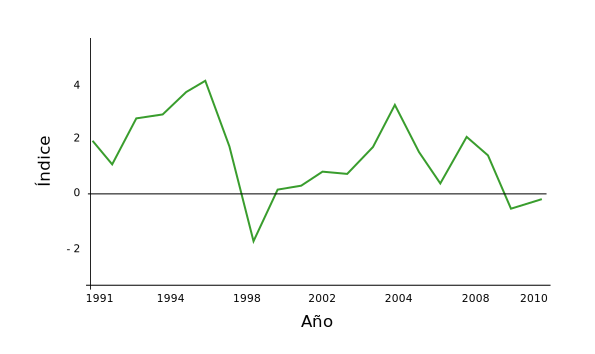
\includegraphics[width=150mm]{capitulos/graficos/AsianCrisis} 
\label{fig:AsianCrisis} 

	\footnotesize
	Fuente: IMF (2.009)

\end{figure}


Al tratarse de un hecho histórico relativamente contemporáneo, todavía hay diferentes puntos de vista sobre las causas de esta crisis, aun así, se va a intentar dar explicación.

El primero, se basa en la teoría desde una perspectiva psicológica. Algunos de los autores relevantes que sostienen esta postura son Radelet y Sachs (1.998), Chang y Velasco (1.999) y Marshall (1.998), y se basan en un cambio de las expectativas debido al contagio regional. Estos autores defienden que, la mayor fuerza causante de esta crisis fue el pánico que surgió entre los inversionistas nacionales e internacionales.

El segundo enfoque, se basa en los fundamentos de los desequilibrios. Como son las distorsiones estructurales, políticas gubernamentales equivocadas y un efecto manada o \emph{herding} \footnote{Concepto definido a lo largo de este capítulo.}.

La tercera visión, está basada en las enormes y rápidas entradas y salidas de capital que fueron devastadoras, junto con los efectos negativos del Yang frente a la moneda extranjera.

Si se mezclan los conceptos de estas tres teorías, se puede apoyar la idea de que una excesiva entrada de dinero va destinada a unos pocos activos, de este modo, infla a éstos por encima de sus valores fundamentales. Si a esto expuesto se le suma que ocurre dentro de una economía que todavía tiene deficiencias estructurales, se puede concluir que estas entradas y salidas monetarias pueden tener unas repercusiones muy graves.

Todo ello se puede apreciar claramente en la Figura \ref{fig:AsianCrisis}.


\subsection{La burbuja punto com}    
Se trata de una de las mayores burbujas del mercado de valores de todos los tiempos que irrumpió en marzo del año 2.000. Más de siete billones de dólares en valores de mercado se evaporaron en tan sólo dos años.

El período viene marcado por la expansión de Internet en la sociedad. Se trataba de una tecnología totalmente revolucionaria que abriría nuevos horizontes. Permitió nuevas posibilidades de negocio, ya que era una novedosa forma de compartir y transmitir información. También proporcionaba nuevas formas de adquirir bienes y servicios. Se le denominó \emph{La Nueva Economía}. Las posibilidades eran ilimitadas, y como tal, se presentaba como un nuevo concepto donde los límites todavía no estaban claros. La retroalimentación positiva comenzó, y en ese momento, los medios de comunicación jugaron un papel muy importante porque supuso un impulso nunca antes visto. Internet no tardó en convertirse en una de las variables más importantes de la vida cotidiana.

Los inversores de capital de riesgo se convirtieron en los principales protagonistas en el inicio del boom. Cuando la primera empresa punto com se hizo popular, el precio de las acciones se disparó automáticamente. Por lo tanto, estos inversores de riesgo modificaron su estrategia habitual y en lugar de centrarse en la viabilidad del proyecto, todos los esfuerzos fueron destinados a que la empresa se hiciese famosa y cobrar así un beneficio rápido y sustancial. En el primer trimestre del año 2.000, 916 empresas invirtieron 15,7 mil millones de dólares en más de mil de las empresas pioneras de Internet, según afirma Malkiel (2.007). Cualquier empresa lo suficientemente popular relacionada con la tecnología, vio como el precio de sus acciones crecía sin cesar.

Uno de los aspectos más relevantes a tener en cuenta, es que los criterios tradicionales de \emph{valoración} para las empresas cambiaron. Los fundamentos económicos, la relación precio y beneficio o las ventas ya no son importantes. Los factores importantes se contabilizaban, y todavía se contabilizan, con el número de visitas que ha tenido la página web, cuanto tiempo lo hicieron, si los internautas visitantes gastaron dinero o simplemente se informan, etc.

\begin{figure}[!h] 
\caption{La burbuja de las punto com} 
\centering 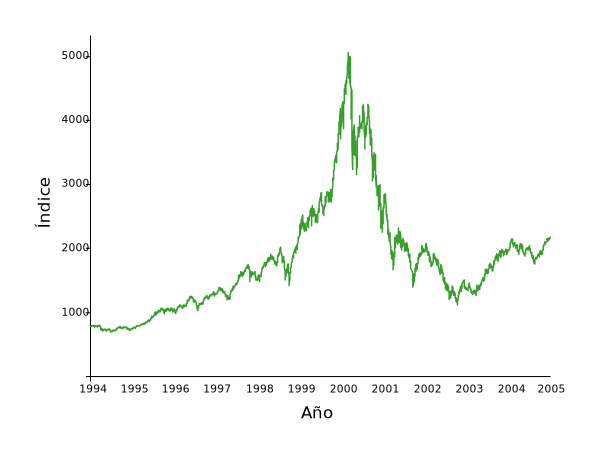
\includegraphics[width=150mm]{capitulos/graficos/comBubble} 
\label{fig:La burbuja de las punto com} 

	\footnotesize
	Fuente: Elaboración propia a partir de los datos recuperado en NASDAQ (2.012)

\end{figure}

Como se puede ver en la Figura \ref{fig:La burbuja de las punto com}, el índice NASDAQ se mantuvo triplicando su valor desde finales de 1.998 hasta marzo de 2.000. La especulación se incrementó enormemente. Comprar por Internet se convirtió en una actividad popular y había más de diez millones de comerciantes al día en Internet. También hubo escándalos fraudulentos como \emph{Enron}. A lo largo de 1.999 y también a principios del año 2.000, la Reserva Federal de Estados Unidos aumentó los tipos de interés seis veces, provocando que la economía perdiese velocidad. Por otro lado, muchas de las empresas que se basaban en Internet para obtener beneficios reportaron grandes pérdidas netas. Eran dos factores importantes para que los inversionistas reinterpretasen sus expectativas.

Cuando la burbuja explotó, más de 8 billones de dólares en valores de mercado, se evaporaron. Incluso las empresas líderes se derrumbaron, algunos ejemplos son: Amazon, Cisco Systems, Corning, JDS Uniphase, Nortel Networks, Priceline, Yahoo.com, entre otros. Todos ellos perdieron entre un 90 y un 99,7 por ciento del precio de las acciones.

\subsection{La burbuja inmobiliaria} 
Esta burbuja se conoce generalmente como la burbuja inmobiliaria, la burbuja de las hipotecas sub-prime o la burbuja de crédito, entre otros nombres. Sin embargo, se puede demostrar que no sólo afectó al sector inmobiliario, sino que también se materializó en otros sectores provocando una crisis global.

En este caso, vamos a centrar el estudio en la burbuja inmobiliaria española aunque no se ha de perder de vista la burbuja inmobiliaria en Estados Unidos.

En primer lugar, se puede plantear la siguiente cuestión, \emph{¿Qué es una burbuja inmobiliaria?} Según el blog de economía Gerencie.com: \emph{una burbuja inmobiliaria es un incremento excesivo e injustificado de los precios de los bienes inmuebles o bienes raíces, ocasionado generalmente por la especulación}.

\begin{figure}[!h] 
\caption{La burbuja inmobiliaria de España. Precio nominal medio de la vivienda nueva en España} 
\centering 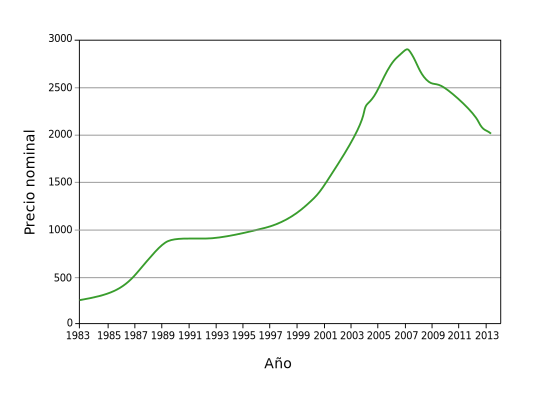
\includegraphics[width=150mm]{capitulos/graficos/precioVivienda} 
\label{fig:precioVivienda} 

	\footnotesize
	Fuente: Wikipedia Española

\end{figure}


\begin{figure}[!h] 
\caption{La burbuja inmobiliaria de Estados Unidos} 
\centering 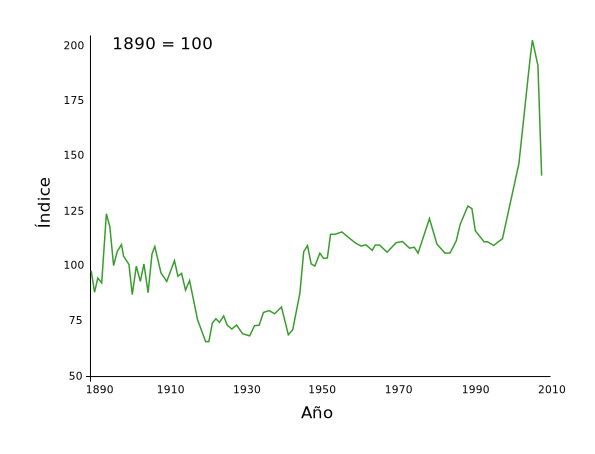
\includegraphics[width=150mm]{capitulos/graficos/HousingBubbleUSA} 
\label{fig:HousingBubbleUSA} 

	\footnotesize
	Fuente: Shiller Index

\end{figure}

Según el autor De la Dehesa (2.009), esta burbuja comenzó a gestarse al finalizar la Segunda Guerra Mundial incrementándose así, década tras década, el precio de la vivienda. Es de esperar que la población no de mayor importancia al hecho de que aumente el precio, ya que se ve como algo natural y se terminan olvidando los fundamentos económicos que refutan el comportamiento cíclico de ésta, es decir, que lo que en un momento dado sube, luego tiende a bajar y todo lo que aumenta abruptamente tiende a caer en exceso.

Una de las variables más condicionantes de la burbuja inmobiliaria es el tipo de interés. Un bajo tipo de interés proporciona una mayor demanda de créditos por parte de los clientes. Pero por otro lado, si los tipos de interés tienen una tasa alta, las entidades bancarias no hubieran concedido créditos a los clientes denominados \emph{NINJA}, probablemente hoy por hoy no se hablaría de crisis económica. En el mercado financiero se conoce a los clientes NINJA como a aquellos que no disponen de ingresos fijos, empleo fijo, o propiedades con las que saldar las deudas concertadas con las entidades bancarias. La palabra \emph{NINJA} es un acrónimo de \emph{No Income, No Job, no Assets}. \footnote{En castellano se traduce como no ingresos, no trabajo, no activos}. Al mismo tiempo, surgió el término \emph{titulización} que según la Real Academia de la lengua Española, titulizar se pude definir como: \emph{convertir determinados activos, generalmente préstamos, en valores negociables en el mercado}\footnote{Diccionario de la Real Academia de la lengua española}.

El antiguo método que empleaba la banca era el de \emph{comprar para mantener}. Este sistema se basaba en que los bancos obtenían su financiación a partir de los depósitos, prestando a su vez a largo plazo a clientes, para mantener las relaciones con éstos hasta el fin de los préstamos, es decir, varios años a posteriori. Las posibles inestabilidades se mitigan con la relación a largo plazo con los clientes, la existencia de sistemas de garantías de depósitos y la función de prestamista de última instancia de los bancos centrales.

Durante la primera década del año 2.000, el sistema da un giro de ciento ochenta grados hacia lo que se denomina \emph{originar para distribuir}. En este nuevo sistema, los bancos son meros intermediarios entre los clientes \footnote{Los potenciales generadores de riesgo de crédito.} y los financiadores \footnote{Los demandantes de dicho riesgo.}. El riesgo inicial existente intrínsecamente, se empaqueta y reestructura hasta conseguir el binomio rentabilidad y riesgo objetivo.

El nuevo sistema implantado, produjo un deterioro de las condiciones crediticias. El sector privado, desarrolló diferentes formas de titularizar hipotecas consiguiendo atraer una enorme cantidad de nuevo capital en la industria. Mientras tanto, el gobierno estaba permitiendo esta situación sin intervenir para garantizar mínimos lógicos de solvencia que respaldase esa operativa. 

El resultado de este cambio fue aportar grandes sumas adicionales de dinero disponible para la compra de viviendas y aumentar el tamaño del sector inmobiliario. Además, se animaba a los propietarios que ya tenían las primeras hipotecas, a que las aumenten o a que realizasen una segunda hipoteca sobre su inmueble para hacer nuevos consumos familiares. De este modo, aumentó fuertemente la cantidad de la deuda asumida por los consumidores. Se puede hacer una analogía afirmando que los consumidores utilizaban sus casas como un cajero automático.

A continuación se van a mostrar dos gráficos. El primero se corresponde con la burbuja inmobiliaria de España y el segundo con la burbuja inmobiliaria de Estados Unidos.

Como se puede comprobar en la Figura \ref{fig:precioVivienda}, en el momento en el que la burbuja estalló, los precios de las viviendas comenzaron a caer secuencialmente en picado. A mediados de 2.009, estos precios disminuyeron en más de un tercio de su máximo histórico. Muchos propietarios, se encontraron con que sus casas valían menos que la cantidad del dinero pactado en sus hipotecas y comenzaron a sucederse los impagos, deteniéndose la concesión de préstamos por parte de las entidades bancarias. Los mercados de crédito se congelaron y se convirtieron en instituciones incapaces de refinanciar su deuda a corto plazo.

Los valores con garantía hipotecaria, se vendieron a lo largo y ancho de todo el mundo, lo que provocó el debilitamiento de todos los sistemas bancarios mundiales. De este modo, se desencadenó una grave recesión mundial, con unas tasas de desempleo muy elevadas y en las que actualmente todavía hay sumergidos innumerables países, no tan sólo es el caso de España.

\section{Análisis descriptivo del concepto burbujas económicas} 
Como se anticipó en el epígrafe 1.2, es evidente que una burbuja puede manifestarse en diversos contextos y en diferentes clases de activos. También se ha podido apreciar que podría dar lugar a un efecto neto positivo como en el caso de la burbuja de la manía del ferrocarril, también a una redistribución de la riqueza como ocurrió en la manía de los tulipanes; o por el contrario sufrir un efecto neto negativo, como en la de Japón. Sin embargo, existen diferentes factores que vale la pena destacar.

\subsection{Factores que influyen en la formación de las burbujas económicas} 

Para comenzar, la primera variable fundamental es el \emph{precio}. Es la característica más notable de una burbuja ya que los precios aumentan enormemente en un corto período de tiempo, perdiendo la correlación con los valores fundamentales y alcanzando en muchas ocasiones precios desorbitadamente altos. Pero finalmente estos precios colapsarán y tendrán como resultado una caída muy abrupta. 

El segundo factor elemental es la \emph{inversión/especulación}. Como se ha podido comprobar a lo largo del capítulo, a cada burbuja van asociadas grandes cantidades de dinero que entran y salen del mercado.

La tercera característica se ha podido apreciar en el epígrafe anterior con la descripción de las burbujas económicas más importantes a lo largo de la historia. La mayoría de éstas, comparten un contexto común en su formación, como es el de una gran \emph{empresa emprendedora}, no tiene que ser como tal una empresa, puede darse como una idea innovadora para la población. Tras la creación de esta \emph{empresa} siempre hay una clara \emph{incertidumbre} sobre la rentabilidad de ésta, de su estrategia de negocios, de su capacidad en los mercados, etc. 

No es conveniente identificar a esta cuarta variable, que es el \emph{apalancamiento financiero}, como un factor en sí de la burbuja económica, pero aun así, se puede decir que el apalancamiento financiero es un término comúnmente conocido y que consiste en recurrir a la deuda para aumentar la rentabilidad de los accionistas \footnote{La rentabilidad financiera}. El posible aumento de la rentabilidad, tiene como contrapartida un aumento del riesgo financiero. Poniendo como ejemplo la burbuja de la Compañía de los Mares del Sur, ésta Compañía aceptó el pago inicial de los accionistas y el resto a pagar en cuotas. Por lo tanto, bien sea a través de pagos iniciales o por la abundancia de crédito, el apalancamiento se encuentra entre los agentes que participan en el proceso de formación de la burbuja.

Existe un quinto agente que es el \emph{gobierno}. En la mayoría de las burbujas económicas, y como se comprobará a lo largo del proyecto, sus respectivos gobiernos participan en diversas etapas de ésta tomando diferentes medidas. Por ejemplo, en el caso de los tulipanes, el gobierno trató de evitar el estallido de la burbuja. Por otro lado, en la burbuja de la Compañía del Mississippi, fue el propio gobierno quien fue gestando la burbuja económica en manos de John Law. 

En resumen, se podría argumentar que una burbuja, ocurre gracias a una perfecta mezcla entre variables importantes del mercado como son la incertidumbre, los tipos de interés, el apalancamiento y la intervención de los gobiernos. De este modo, los flujos de dinero masivos que se introducen en las burbujas provocan que los precios se disparen.

\subsection{Etapas de una burbuja económica}

Cada una de las burbujas económicas expuestas a lo largo del capítulo, ha quedado ilustrada por un gráfico. Independientemente de cuál de ellas se elija para apreciar la evolución de los precios, se puede valorar la similitud de la campana. Según el jefe del departamento de estudios globales, de la Universidad de Hofstra, El Dr. Jean-Paul Rodrigue, las principales etapas de una burbuja se pueden apreciar en la siguiente Figura \ref{fig:bubbleFases}:

\begin{figure}[!h] 
\caption{Fases de una burbuja económica} 
\centering 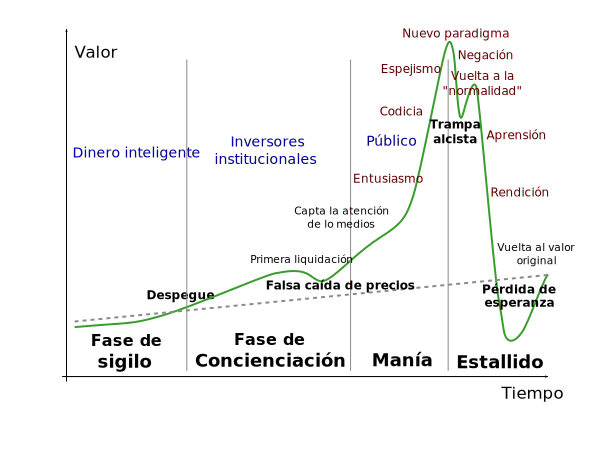
\includegraphics[width=150mm]{capitulos/graficos/bubbleFases} 
\label{fig:bubbleFases} 

	\footnotesize
	Fuente: Rodrigue (2.010)

\end{figure}


De una forma teórica, se pueden clasificar estas fases en:
\begin{enumerate}
	\item \emph{Sigilo}. Pocos inversionistas especializados se percatan de la revalorización sustancial y asumen el riesgo de ser pioneros. A este hecho, se le denomina \emph{dinero inteligente}, ya que introducen dinero en el mercado con cautela para que los demás participantes lo noten. Este tipo de inversionistas, pueden tener una información más fiable y más rápida, así como herramientas y conocimientos necesarios para afrontar los hechos en el mercado. Los precios de los activos se incrementarán gradualmente y sin la participación de los inversores masivos. El dinero inteligente, también ganará posiciones poco a poco.
	\item \emph{Concienciación}. La introducción de dinero realizada en la anterior etapa, es detectada por otros inversores que ponen más dinero sobre los activos y los empujan al alza. Nuevos inversores pueden adquirir los primeros beneficios provocando un aumento gradual del precio. Al final de esta etapa, los medios de comunicación se involucran y como resultado, el resto de inversores se introducen en el mercado. 
	\item \emph{Manía}. La tendencia de los precios es claramente al alza y los ciudadanos deciden invertir sus ahorros para poder percibir hipotéticos grandes beneficios en un futuro. Estás importantes cantidades de capital, generan expectativas aún mayores y alimentan los precios para que éstos aumenten. Sin embargo, el dinero inteligente invertido en la primera fase, junto con los inversores institucionales, se encuentra en \emph{silencio}, mientras que la venta de los activos está sobrevaluada para el resto de la ciudadanía inversora.

	Durante este periodo de \emph{locura}, todo el mundo trata de participar aunque no se tengan los conocimientos y la preparación adecuada para llevar a cabo transacciones inteligentes. Cuando el crédito es accesible y barato, esta fase dura mucho más tiempo de lo esperado. En este intervalo de tiempo, los medios de comunicación toman parte de la burbuja asegurando a los inversores que los precios han alcanzado una \emph{meseta permanente} con el fin de justificar los precios vertiginosos. La burbuja se comienza a volver más hostil y se encuentra a punto de eclosionar. 
	\item \emph{Estallido}. En un momento determinado y más o menos al mismo tiempo, todos los agentes implicados en el mercado se dan cuenta de que la situación ha cambiado. Aparece la desconfianza y el sentimiento de que las expectativas se desmoronan. Hay una etapa de negación, donde muchos inversores, embelesados por el mercado, tratan de convencer a todos de que el retroceso es sólo temporal. Este hecho provoca un pequeño resurgimiento, pero el espejismo tarda poco en desaparecer. Los descensos se desencadenan a cada cual más espectacular. El colapso se hace factible y los inversores en general se tienen que quedar con los activos sobrevalorados, mientras que el dinero inteligente, invertido en la primera fase, había dejado el mercado hace mucho tiempo. 
	
	Muchos agentes aprovechan la quiebra para adquirir este tipo de activos, ya que se produce una oleada de ventas a precios muy bajos. Sin embargo, la gente en ese momento, considera que estos activos están contaminados y es cuando vuelve a aparecer el dinero inteligente adquiriendo gangas a precios muy bajos.
\end{enumerate}

Es interesante destacar que los primeros en abordar el mercado, son los individuos con \emph{dinero inteligente}. Este tipo de inversionistas podrían tener algún tipo de monopolio en cuanto a información se refiere. Los segundos a tomar posiciones, son los inversores institucionales, lo que provoca la llamada de atención de los medios de comunicación quienes entran en juego a lo largo de la manía. 

\section{Diferentes teorías sobre las burbujas económicas}
En esta sección, se presentan las teorías sociales y psicológicas más relevantes que existen sobre las burbujas económicas.

Una de las teorías más sorprendentes, es la de la inexistencia de burbujas económicas defendida por Peter Garber (2.000). Para poder comprender la postura de este autor, hay que destacar la hipótesis de los mercados eficientes, a partir de ahora denominada: \emph{EHM} y que Peter Garber (1.990) la define como, \emph{la idea de que los precios que prevalecen en el mercado, hacen que sea imposible ganar unos beneficios económicos anormales provenientes de la propia negociación en ese mercado}. Esto quiere decir que en un mercado eficiente todos los bienes o títulos estarán perfectamente valorados, lo que evitará la aparición de sobre o infravaloración de los mismos. Esto tendrá como resultado que los inversores obtendrán un rendimiento sobre su inversión apropiada al nivel de riesgo asumido, ya que no es posible superar los resultados del mercado excepto a través de información privilegiada o de la suerte. Es por esta razón, por la que siempre hay inversionistas buscando información que les permita pronosticar con precisión los precios futuros del bien.


Garber defiende que los inversionistas basan sus decisiones en la percepción sobre los fundamentos del mercado. Si se da este caso, entonces el precio de la acción debe reflejar todos los factores fundamentales, y de acuerdo con la EHM y la definición de burbuja económica, se obtiene como resultado que las burbujas económicas en sí mismas no pueden existir. Por lo que este autor llega a la conclusión de que \emph{las burbujas están en divergencia con cualquier información económica razonable}.

Garber, también defiende que la especulación es meramente un factor psicológico pese a que se le puede dar un sentido económico y lo ilustra con las burbujas de la Compañía del Mississippi y de la Compañía de los Mares del Sur.  Ambos proyectos macroeconómicos llevados a cabo por los gobiernos de Francia y de Londres respectivamente, fracasaron porque tuvieron partes defectuosas dentro del plan ideado y porque los economistas de aquellos años, respaldados por estos gobiernos, no trabajaron día a día en las herramientas financieras que debían. Para los economistas no es de buen gusto aceptar que un \emph{experimento} ha fallado. 

En cuanto a los factores psicológicos se refiere, es importante señalar que proporcionan valiosa información y se consideran buenos indicadores a tener en cuenta en el tema a tratar. Esta teorías psicológicas serán desarrolladas a lo largo de este epígrafe, y tienen su base en el concepto psicológico keynesiano que desarrolló John Maynard Keynes (1.935), y al cual denominó \emph{espíritus animales,} 	\footnote{Texto ampliado en el Anexo 1} en su obra maestra \emph{La teoría general de la ocupación, los intereses y el dinero}, que fue publicado en 1.935. Por lo tanto, se han de dar unas pinceladas keynesianas como base.

Keynes habla de \emph{espíritus animales} como un término que describe los sentimientos que influyen en el ser humano y en su comportamiento, y que a su vez pueden ser mensurables en términos de \emph{confianza de los consumidores}	\footnote{Se trata de un indicador económico que mide el grado de optimismo que los consumidores perciben sobre el estado del mercado y sobre su propia situación financiera personal.} que ésta a su vez también puede ser medida por los \emph{espíritus animales}. Los inversores en general se suponen demasiado ignorantes para formar estimaciones fiables de los valores actuales. \emph{Su ignorancia conduce a la negociación a corto plazo y a la especulación}. Keynes concluye definiendo la expresión espíritus animales como \emph{el impulso espontáneo de la acción en lugar de la falta de acción} \footnote{Keynes, J. (1.935)}. Creía que, las acciones inducidas por este espíritu animal, eran producidas por la irracionalidad humana.
Con esta breve explicación de la teoría de Keynes se va a proceder a explicar cuatro teorías psicológicas.

\subsection{La teoría del más tonto}

Según esta teoría, defendida entre otros por Peter Garber (2.000), a los agentes del mercado que tienen un optimismo elevado en las acciones, se les denomina los tontos. Éstos se encargan de comprar activos sobrevaluados, con la intención de venderlos a un precio aún más alto a otros agentes del mercado - denominados los más tontos ya que tiene expectativas aún más altas que los anteriores o demasiado optimistas sobre los precios de los activos - y están dispuestos a especular con ellos porque creen que el precio no refleja el valor fundamental. El ciclo continúa con los tontos y los más tontos en el mercado hasta que la burbuja estalla cuando ya no hay más tontos dispuestos a comprar al precio máximo. 

\subsection{La teoría del comportamiento de manada} 

Este término proviene del concepto de pastoreo. Y no es más que un símil entre el comportamiento animal y el comportamiento humano. Esta teoría, apoyada por Peter Garber, afirma que las personas imitan las acciones, bien sean racionales o irracionales, de un grupo más grande de individuos. Es decir, la multitud de inversores compran y venden según se mueva el mercado.

Los análisis técnicos de mercado, se basan generalmente en este concepto, ya que su objetivo principal es detectar las tendencias del mercado, es decir, el comportamiento de manada para \emph{asegurar} inversiones. Este hecho no sólo se puede dar como figura individual, si no que también existen inversionistas institucionales como los fondos de inversión que también lo utilizan.

Para poder comprender dicha teoría de una forma sencilla y clara, se va a realizar una comparativa con un banco de peces. En un banco de peces, todos los miembros se decantan por seguir la dirección que toman los demás en su conjunto, sin una coordinación ni organización determinada. De este modo, en un mercado alcista, los inversores seguirán la tendencia especuladora hasta que ésta sea insostenible. En ese momento, el mercado procurará dar un giro de ciento ochenta grados para que los inversores comiencen a vender causando entonces, una caída brusca en el precio y dando lugar al final de la burbuja. Esta teoría del comportamiento gregario se da en otros aspectos de la vida humana como por ejemplo las modas. 

\subsection{La teoría de la extrapolación} 

El aspecto clave de la extrapolación de datos históricos, según los autores Fisher  \& Statman (2.002), se proyecta hacia el futuro con la base de que lo que ha ocurrido con ciertas condiciones, se va a repetir en un futuro que tenga el mismo contexto. En el caso de las burbujas se suele llevar a cabo una extrapolación de precios manteniendo la creencia de que  éstos continuarán su tendencia pasada en el futuro. El apoyo de este argumento proviene del hecho de que los inversores tienden a asociar los últimos rendimientos de determinados activos con retornos futuros, a la consecuencia de sobrepujar algunos activos de riesgo con el fin de mantener y alcanzar las mismas tasas del pasado. Sin embargo, este proceso conduce a un punto en que los beneficios ya no son positivos y los inversores no se sienten compensados  por el riesgo y se sucede el estallido de la burbuja.

\subsection{La teoría del riesgo moral}

Para poder explicar esta teoría se va a proceder a dar un ejemplo ilustrativo con el nivel de seguridad que puede haber en una casa. Este ejemplo ha sido recuperado de Wikipedia.

En una casa, los propietarios pueden decidir instalar una puerta acorazada, reduciendo así el riesgo de robo. Al mismo tiempo pueden ir reduciendo este tipo de riesgos hasta que las ganancias marginales de tomar precauciones sean iguales que los costes marginales de éstas, es decir, hasta que se obtenga mayor beneficio por cada precaución que se tome. Sin embargo, si los propietarios tienen concertado un seguro de hogar en el que se cubre el robo íntegro de la casa, tendrá menos incentivos instalar la puerta acorazada y aumentar así, la probabilidad de que se produzca un robo. 

Por lo tanto, en términos económicos, se podría definir el riesgo moral como, cada movimiento que altera la relación rentabilidad y riesgo. Si se da el hecho de que el agente que asume el riesgo sufre una situación fatal, entonces éste consigue un incentivo para adquirir un nivel de riesgo por encima de sus posibilidades. De este modo puede generar la inestabilidad del sistema y la burbuja económica podría surgir como una consecuencia.



\section{¿Puede ser positiva la existencia de una burbuja económica en la sociedad?} 
En este epígrafe, se discutirá si las burbujas tienen efectos positivos o efectos negativos sobre el bienestar económico general y se explicarán las posibles consecuencias. 

Como se ha mencionado anteriormente, no todas las burbujas son negativas ya que se necesitan ciertos tipos específicos de éstas en nuestro sistema monetario. Por ejemplo, algunas pueden conducir a una expansión de los sectores económicos que sin su existencia nunca hubiesen tenido lugar. 

Se va a estudiar en qué momento es más conveniente o inconveniente actuar, es decir, en el inicio, durante o en su defecto, y si se diese el caso, antes de la burbuja porque existan signos claros de ésta, o por el contrario después del estallido.

\subsection{Burbujas económicas positivas}

En primer lugar, convendría dar explicación acerca de lo que es el \emph{dinero fiduciario}, para ello se puede decir que el dinero fiduciario tiene su fundamento en la confianza de la ciudadanía sobre esa moneda y en las entidades encargadas de emitirla, ya que ésta no tiene respaldo material.

A la hora de catalogar al dinero fiduciario como una de las mayores burbujas económicas en si mismas, se tiene que tener en cuenta que su valor fundamental es cero. En el año 1.971, el entonces presidente de los Estados Unidos Richard Nixon, eliminó la convertibilidad del patrón oro, lo que supuso la pérdida de relación entre el dinero papel y el tan codiciado metal. Entonces se puede plantear una pregunta, \emph{¿Qué podría asignar valor al dinero de una forma completamente arbitraria?} La respuesta es: la confianza y comodidad. 

Según Samuelson (1.958), \emph{la confianza} que confiere el dinero, permite intercambiar a los agentes, bienes y servicios con la garantía y respaldo del Banco Central. Y por otro lado, \emph{la comodidad} que aporta el dinero fiduciario, ya que éste sirve como un medio de intercambio. Y por último, destacar que este tipo de dinero se utiliza para pagar  impuestos, lo que le otorga un valor añadido.

De todas las burbujas expuestas a lo largo del capítulo, los dos mejores ejemplos que representan el espíritu positivo de una burbuja económica, en cuanto a la expansión de los sectores económicos se refiere, es sin duda la manía del ferrocarril. Un total de 10.000 kilómetros fueron construidos como resultado de los proyectos autorizados entre 1.844 y 1.846. Y en segundo lugar, la burbuja punto com, ya que amplió los sectores de telecomunicaciones e introdujo a la población en la nueva era de Internet. 

\subsection{Burbujas económicas negativas}

Tirole (1.985), es uno de los primeros autores que afirmó que las burbujas económicas tenían efectos divergentes en diferentes modelos económicos. También defiende que, al comienzo de la burbuja económica, los compradores y vendedores se introducen en el mercado con un conjunto de informaciones comunes y por lo tanto el conocimiento general es homogéneo, reina la racionalidad y los recursos son asignados eficientemente antes de las negociaciones. También argumenta que tan sólo unos pocos agentes pueden realizar compras y ventas de forma infinita.

Hay que destacar que al autor Peter Diamond (1.965), defiende que uno de los motivos de la existencia de las burbujas puede ser la infinidad de hogares que pueden negociar con activos financieros. Pese a esta teoría, defiende que una burbuja, sólo se le podrá denominar como tal, cuando crezca al mismo tiempo y de la misma forma que el resto del mercado. 

Como conclusión, se puede decir que para poder considerar que una burbuja económica es una burbuja en sí misma, el mercado ha de crecer de menara diferente a los ratios que se consideran apropiados, y a su vez, poseer una enorme acumulación de capital. Para poder comprender el crecimiento paralelo con el mercado, cabe destacar la definición de \emph{burbuja asintótica}: \emph{Se trata de una burbuja que crece al mismo tiempo que lo hace el resto de la economía, teniendo en cuenta que el consumo es eficiente}.	\footnote{Diamond, (1.965)}

A posteriori, los autores Saint-Paul (1.992), Grossman Yanagawa (1.992)y King And Ferguson (1.993), modifican la teoría de Diamond defendiendo que las burbujas pueden darse sin la existencia de una entrada de capital excesiva, argumentando así, que estos niveles de capital dependen de la productividad. Concretamente los autores Grossman y Yanagawa (1.992) ampliaron algunos modelos de Tirole para incluir a las economías que crecían en el largo plazo y a una tasa endógena. La conclusión a la que llegaron en su tesis fue que \emph{las burbujas retardan el crecimiento de la economía, posiblemente incluso en el largo plazo y reducen el bienestar de todas las generaciones nacidas tras la burbuja económica}. Concluyen también, afirmando que el impacto de la explosión de la burbuja, podría ser beneficioso para la generación actual pero puede tener graves consecuencias futuras ya que retarda el crecimiento económico para éstas.

Los mejores ejemplos de este tipo de burbujas económicas son las inmobiliarias, ya que es la clase de burbuja más cercana en el tiempo y además, un gran número de importantes economías mundiales occidentales están inmersas en ella. 

Una vez realizado este análisis en profundidad de qué es una burbuja económica en todos sus sentidos, se va a proceder a explicar tres de las burbujas más relevantes de la historia. En el capítulo dos se desarrollará a la tulipomanía, en el capítulo tres se introducirán la burbuja de la Compañía del Mississippi y el sistema de John Law y para finalizar se explicará la burbuja de la Compañía de los Mares del Sur, sustancialmente ligada a la desarrollada en el capítulo tres. 

